%------------------------------------------------------------------------------
% This is a LaTeX template for the scientific justification of IRAM Proposals 
%------------------------------------------------------------------------------
% 
% We encourage IRAM proposers to use this template for the sake of unity 
% and clarity when Program Committee members assess their proposals.
% 
% You may customize this template to suit your preferences (e.g. using BibTex),
% but please respect the following requirements:
%     The scientific and technical justification should contain a 
%     maximum of 2 pages of text (4 pages for Large Programs), 
%     plus 2 pages of Figs., Tables and Refs.
%     The font size should be 11pt or larger.
%
% For Large Programs, the following sections should be included: 
%   i) Scientific Rationale, 
%  ii) Immediate Objective, 
% iii) Feasibility and Technical Justification, and 
%  iv) Organizational Issues.
%
%
%------------------------------------------------------------------------------
%
\documentclass[11pt,a4paper,twoside,graphicx,color]{article}
%
\usepackage[margin=2cm]{geometry}
\usepackage[margin=2cm]{geometry}
\usepackage[pdftex]{graphicx}
\usepackage{color}
\usepackage{txfonts}
\usepackage{paralist}
\usepackage[numbers]{natbib}
\setlength{\bibsep}{0.0pt}
\usepackage{amssymb}
\usepackage[breaklinks, colorlinks, citecolor=blue, linkcolor=MyBlue, urlcolor=RoyalPurple, colorlinks=true, linkcolor=blue, debug, baseurl=' ']{hyperref}
%
% Page size and text dimensions
% Do not change!
\textheight 260mm
\textwidth 178mm
\oddsidemargin -8mm
\evensidemargin -8mm
\marginparwidth 50pt
\topmargin -22mm
\brokenpenalty=10000
\sloppy
%
\bibpunct{(}{)}{;}{a}{}{,} 
\bibliographystyle{aa}
\definecolor{gris}{gray}{0.75}
%-------------------------------------------------------------------
\begin{document}
%
%
\begin{center}{\huge \bf
%-------------------------------------------------------------------
Kinetic Sunyaev-Zel'Dovich mapping towards MACS~J0717.5+3745 (NIKA GT)
%-------------------------------------------------------------------
}\end{center}
%
\centerline{\bf P.I.: R\'emi Adam \& Barbara Comis}
%\paragraph*{Proposal history (shown here but will be put only in the IRAM PMS)}
%The cluster of galaxies MACS J0717.5+3745 has been observed during the first NIKA open pool (February 2014) via the Sunyaev-Zel'Dovich (SZ) effect. In addition to the 150 GHz map, which was the original goal, we have also been able to produce a map at 260 GHz that shows hints of the presence of a significant kinetic SZ signal, as expected for this cluster.

%\paragraph*{Abstract (shown here but will be put only in the IRAM PMS)}
%Measuring the velocity distribution of galaxy clusters provides a precious insight into the physics of mergers, from which large scale structures form in the Universe. In this proposal, we aim at obtaining such observation by pushing further the Sunyaev-Zel'Dovich (SZ) mapping of MACS J0717.5+3745. Observed at both NIKA frequencies, we will derive the first thermal + kinetic SZ mapping in a cluster of galaxies. Combining our maps with extra dataset (mainly X-ray) will allow us to obtain, for the first time, a map of the gas line-of-sight velocity from SZ observations. We will use 3' x 6' OTF scans for a total of 36 hours of observation.

\section{Scientific context}
\paragraph{\large Introduction}
%========== Why measuring cluster velocity: clusters trace both mass and velocity distribution
{\bf Clusters of galaxies} are now widely used to constrain cosmology, thanks to the progress achieved in relating their direct observables to their total mass. In addition to the clusters masses, it is crucial to measure their peculiar velocities as the latter provides a complementary probe to constrain structure formation and its dynamics. Such measurements also allow for the breaking of parameter degeneracies inherent to other cosmological probes. As clusters of galaxies generally form by the gravitational merger of smaller clusters and groups, measuring the {\bf velocity distribution of merging systems} provides insights of the cluster physics, such as shocks in the intracluster medium (ICM), kinematics of the mergers, or hydrodynamical interactions between cluster cores and less dense shock heated regions. In turn, the understanding of these processes can help to relate the cluster observables to their mass, reducing scatter and biases which arise when complex physics is ignored when used for cosmological purposes. However, classical methods (redshift-based surveys) also require an independent distance measurement to subtract the Hubble flow at the object position in order to measure their peculiar velocities, and are therefore limited to small redshifts as the errors scale with distance. 

%========== How measuring cluster velocity: can be probed with SZ
In this proposal, we will use the {\bf Sunyaev-Zel'Dovich (SZ) effect}, to measure both the mass and the velocity of a cluster in an independent manner. We can distinguish the thermal SZ (tSZ) effect, for which the Cosmic Microwave Background (CMB) photons are spectrally distorted by the electronic thermal pressure of the ICM, from the kinetic SZ (kSZ) effect, arising from the CMB Doppler shift induced by the relative motion of the cluster electrons. The kSZ effect is subdominant unless the gas velocity reaches a few tenths of a percent of the speed of light ($\sim$1000~km/s). The expected flux surface brightness is related to the ICM gas pressure in the case of the tSZ effect, and to both the density and the line-of-sight component of the velocity for the kSZ \citep{birkinshaw1999}. The spectral dependence of the tSZ and kSZ effects are given in Fig.~\ref{fig:spectra}. While tSZ probes shocks in mergers from overpressure~\citep[{\it e.g.} \mbox{RX~J1347.5-1145},][]{adam2013}, the kSZ effect is sensitive to the line-of-sight merger motion, being a direct probe of the electron bulk motion. This complements the optical observations which measure the velocity of the individual galaxies, giving a proxy for that of dark matter. Finally, unlike classical probes, the SZ effect observable is not the cluster itself but CMB photons, therefore, it does not suffer from cosmological dimming and is only limited by observational angular resolution and sensitivity.

%%%%%%%%%%%%%%%%%%%%%%%%%%%%%%%%%%%%%%%%%%%%%%%%
\paragraph{\large Targeting the kSZ effect}
%========== MACS J0717.5+3745
The cluster \mbox{\bf MACS~J0717.5+3745}, at $z=0.55$, is a striking example of a merging system. It is a {\bf triple merger} made of four main optically identified groups (Fig.~\ref{fig:maps}, top left) that have {\bf exceptionally large relative line-of-sight velocities} (see Fig.~\ref{fig:spectra}). Using \mbox{X-ray} and optical observations and accounting for the spectral dependences of the SZ effect, we have estimated the expected signal in the NIKA bands (middle row of Fig.~\ref{fig:maps} based on \cite{ruppin2013}). In contrast to a pure tSZ signal, the ratio of the flux density between the two bands is not constant over the cluster extension. Instead, we observe independent regions with a typical size of a few tens of arcsec. Since the signature of the kSZ in \mbox{MACS~J0717.5+3745} is expected to vary in the different regions of the cluster, its measurement will be insensitive to the overall calibration systematic errors.

%========== BOLOCAM
Recently, \cite{sayers2013} have marginally detected the kSZ signal from a single cluster, \mbox{MACS~J0717.5+3745}, with 40 hours Bolocam+CSO observations at 140 and 268~GHz having 58 and 31 arcsec angular resolution, respectively (see also \cite{mroczkowski2012} for the first Bolocam and MUSTANG+GBT SZ data). As Bolocam beams are larger than the signal typical size, their detection is only significant when using a model dependent analysis, {\it i.e.} 4.2$\sigma$, while it reduces to 2.9$\sigma$ when directly using their deconvolved maps. For NIKA, the observing bands are similar but the beams are three times smaller, allowing us to have the {\bf first direct detection of kSZ}.

%========== Proposal history
During the first NIKA open pool of Feb. 2014, we have {\bf already observed {\mbox MACS~J0717.5+3745}} for about 10 hours. These more than successful observations were designed to map the cluster at 150~GHz in order to study its morphology. Thanks to NIKA's excellent performance, we have been also able to produce a 260~GHz map. As the noise is higher at 260~GHz, the {\bf significance of these previous observations is not sufficient to map the kSZ emission} with a peak signal to noise of $\sim 3\sigma$ at this frequency. Nevertheless, we find the recovered signal to be much more consistent with a tSZ+kSZ scenario than with a tSZ-only model. This is shown in the bottom row of Fig.~\ref{fig:maps} where we present the two NIKA maps (not proportional to one another over the cluster extension), that can be compared to the middle row showing tSZ+kSZ model maps.

%========== Conclusion: let's observe the cluster
According to its expected physical properties, to the data we already have in hand and to Bolocam results, {\bf \mbox{MACS~J0717.5+3745} is therefore an ideal candidate to map the kSZ effect}, for the first time, in a cluster of galaxy at sub-arcmin angular resolution.

%%%%%%%%%%%%%%%%%%%%%%%%%%%%%%%%%%%%%%%%%%%%%%%%
%%%%%%%%%%%%%%%%%%%%%%%%%%%%%%%%%%%%%%%%%%%%%%%%
%%%%%%%%%%%%%%%%%%%%%%%%%%%%%%%%%%%%%%%%%%%%%%%%
\section{Technical justification}
\paragraph{\large Ongoing NIKA pilot study/proposed observations}
%========== History
These observations will be part of a pilot study aiming at studying the NIKA2 possibilities for future large programs in terms of SZ science. In addition to \mbox{RX~J1347.5+3745} observed during technical time~\citep{adam2013}, the cluster \mbox{CL~J1226.9+3332} at $z=0.89$ (observed in February 2014) is currently being analyzed to characterize the outcomes of high-redshift cluster observations with NIKA~\citep{CL2014}. Furthermore, three relaxed clusters discovered by Planck will be observed in November 2014 (summer NIKA GT). The study of the kSZ effect with NIKA will complement these tSZ-only observations.

%========== What we will do
In this proposal, we aim at mapping the SZ signal towards \mbox{MACS~J0717.5+3745} at both 150 and 260 GHz (mostly 260~GHz as the 150~GHz map is already good enough) in order to obtain the first tSZ+kSZ mapping of the SZ effect. Combined with extra publicly available \mbox{X-ray} data, allowing temperature estimates, this map will be used to derive the first line-of-sight electron velocity map measured in a galaxy cluster from the kSZ effect. High quality tSZ+kSZ data will be necessary to deal with degeneracies between tSZ relativistic corrections and the kSZ effect.

%%%%%%%%%%%%%%%%%%%%%%%%%%%%%%%%%%%%%%%%%%%%%%%%
\paragraph{\large Towards a tSZ+kSZ mapping}
%========== Spectral index map
Obviously, at least two frequency bands are needed for breaking the tSZ/kSZ degeneracy. For a given pixel on the map, the measured intensity is written as $\Delta~I~(\nu)~=~\alpha~\Delta~I_{tSZ}(\nu)~+~\beta~I_{kSZ}(\nu)$. Using the NIKA observations we can obtain the set of coefficients $\left(\alpha \pm \delta \alpha, \beta \pm \delta \beta\right)$, which will {\bf constrain the amplitude of each tSZ and kSZ components}. The signal to noise of the reconstructed $\alpha$ and $\beta$ maps will of course depend on the signal strength. Assuming 22~arcsec map pixels and fluxes densities similar to those measured with the data we already have at our disposal, we need a root mean square (rms) of 0.25~mJy/beam at 260~GHz to produce a kSZ/tSZ mapping at more than 3$\sigma$. Figure~\ref{fig:spectra} shows the corresponding expected constraints towards regions A, B, C and D.

%========== Velocity
Once the parameters $\alpha$ and $\beta$ are measured, they can be related to the line-of-sight velocity distribution, $v_z$. One needs an extra constraint to break the degeneracy between the density $n_e$, the pressure $P_e$ and $v_z$. To do so we will use available \mbox{X-ray} spectroscopy data ({\it e.g.} Chandra, XMM) that provide temperature and pressure maps ($P_e = n_e k_B T_e$), as done in \cite{mroczkowski2012} but with new deeper Chandra data for better constraints on the ICM. From that point, only little assumption on the gas distribution, that can be estimated from \mbox{X-ray} number count, will be necessary to obtain a map of $v_z$. The possible contamination resulting from lensed background submm sources will be constrained, as done in \cite{sayers2013}, using available deep Herschel/Spire data at 250, 350 and 500 $\mu$m.

%%%%%%%%%%%%%%%%%%%%%%%%%%%%%%%%%%%%%%%%%%%%%%%%
\paragraph{\large Time estimates and scanning strategy}
As discussed above, the 260~GHz data limits the analysis, so we focus only on this band for the required time estimates. We followed the IRAM guidelines given in~\cite{billot2014} to estimate observing times. The sensitivity of the NIKA camera is expected to be 35~mJy s$^{1/2}$ at 260~GHz and 14~mJy~s$^{1/2}$ at 150~GHz~\citep{catalano2014, billot2014}. As done in Feb. 2014, we will use {\bf on-the-fly scans of 6 $\times$ 3 arcmin} alternating along the azimuth and elevation directions. This will allow us to properly define the zero level of our map and ensure the recovery of the signal at scales larger than the subclusters structures. About one third of the observing time will be spent on the core of the signal. We assume a filtering factor of 1.5, based on previous observations for which we obtained a rms of 0.5 mJy/beam at the center of the map in 10 hours, including overhead. Therefore, we expect the noise rms at the cluster peak to scale as $\frac{1.5 \times 35}{\sqrt{3600/3}} \sqrt{1 \ {\rm hour} / t} = 1.5 \times \sqrt{1 \ {\rm hour} / t}$ mJy/beam at 260~GHz. Since we want to recover diffuse faint signal, down to $\lesssim$ 1 mJy/beam, the atmospheric conditions need to be good. We need very {\bf stable weather} and a p.w.v $<$ 2~mm so that $\tau_{225\ {\rm GHz}} < 0.09$. In the case of SZ observations, we assume calibration overheads (focus, pointing, photometry) to account for not more than 25 percent of the overall observing time, similarly to the winter pool of Feb. 2014. Therefore, we request {\bf 36 hours} of observation of \mbox{MACS~J0717.5+3745}, including overheads, to reach the goal rms of 0.25~mJy/beam at 260~GHz when added to our already observed 10 hours. Similarly, at 150~GHz we expect 0.1~mJy/beam rms. The two data sets will also allow for cross checks of our results.

\newpage
\section{Supporting material}
\begin{figure}[h!]
	\centering
	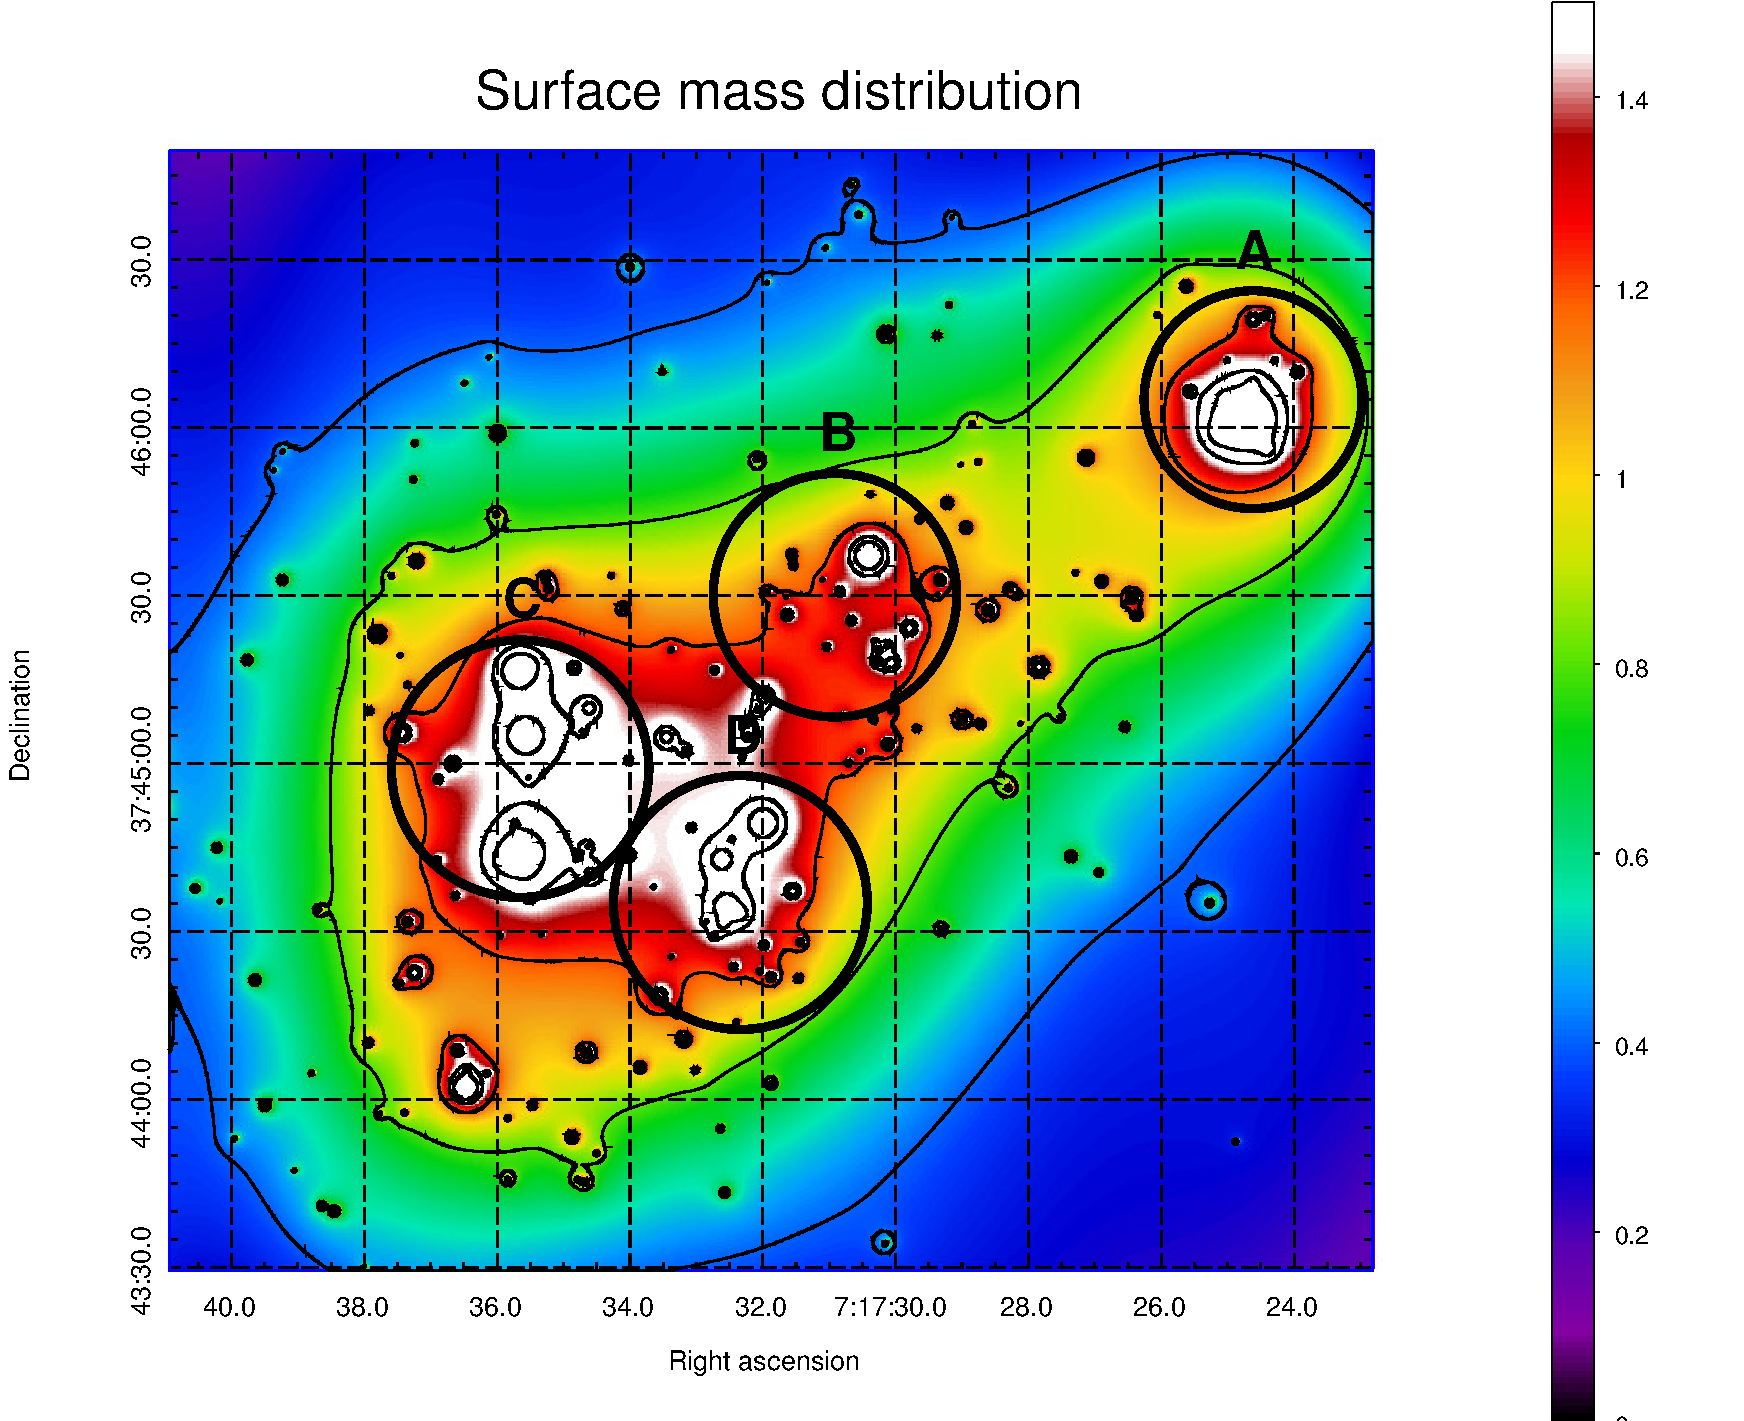
\includegraphics[width=0.42\textwidth]{Lensing.pdf}
	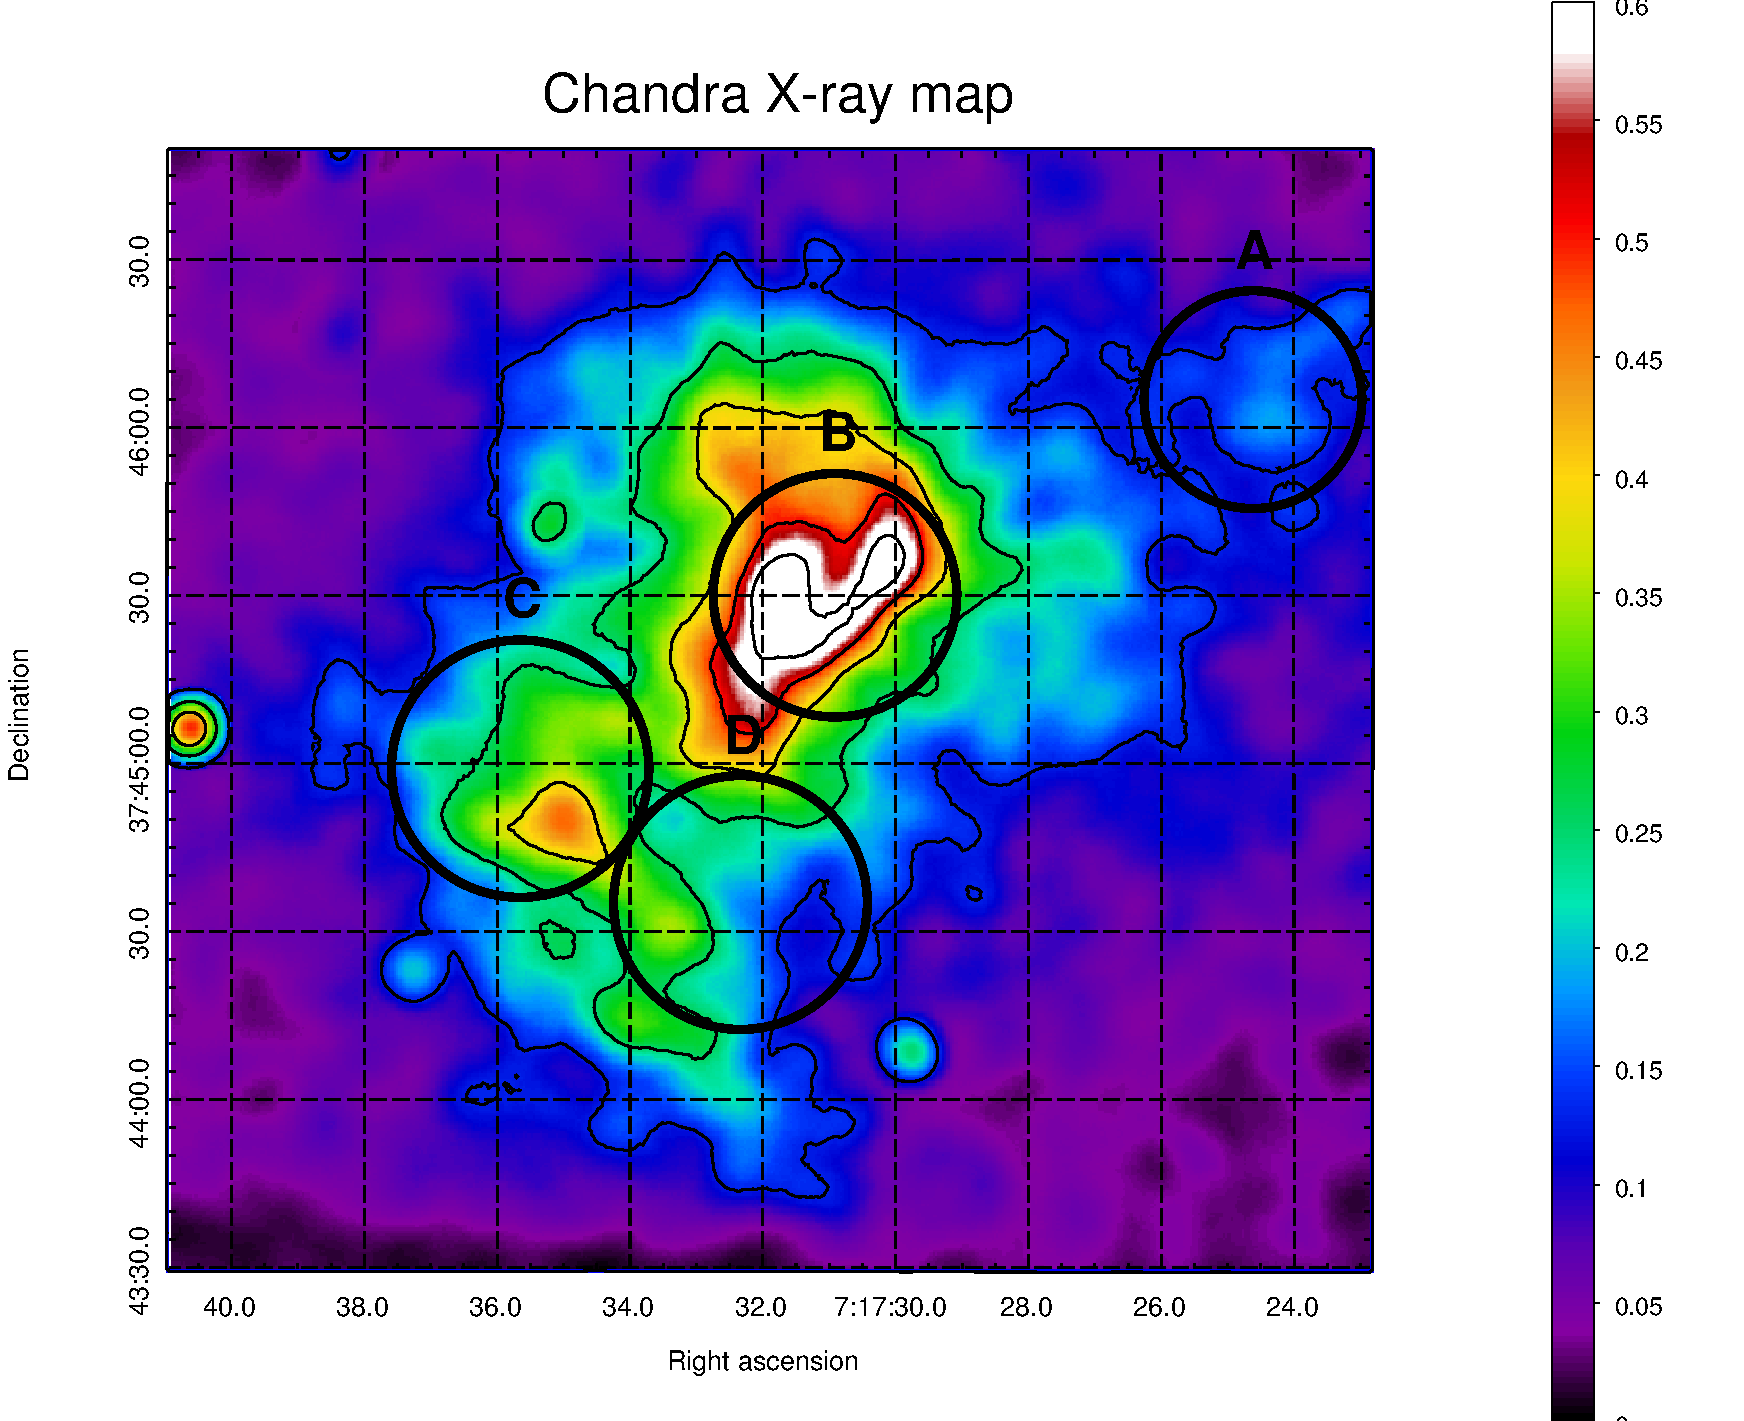
\includegraphics[width=0.42\textwidth]{Xray.pdf}
	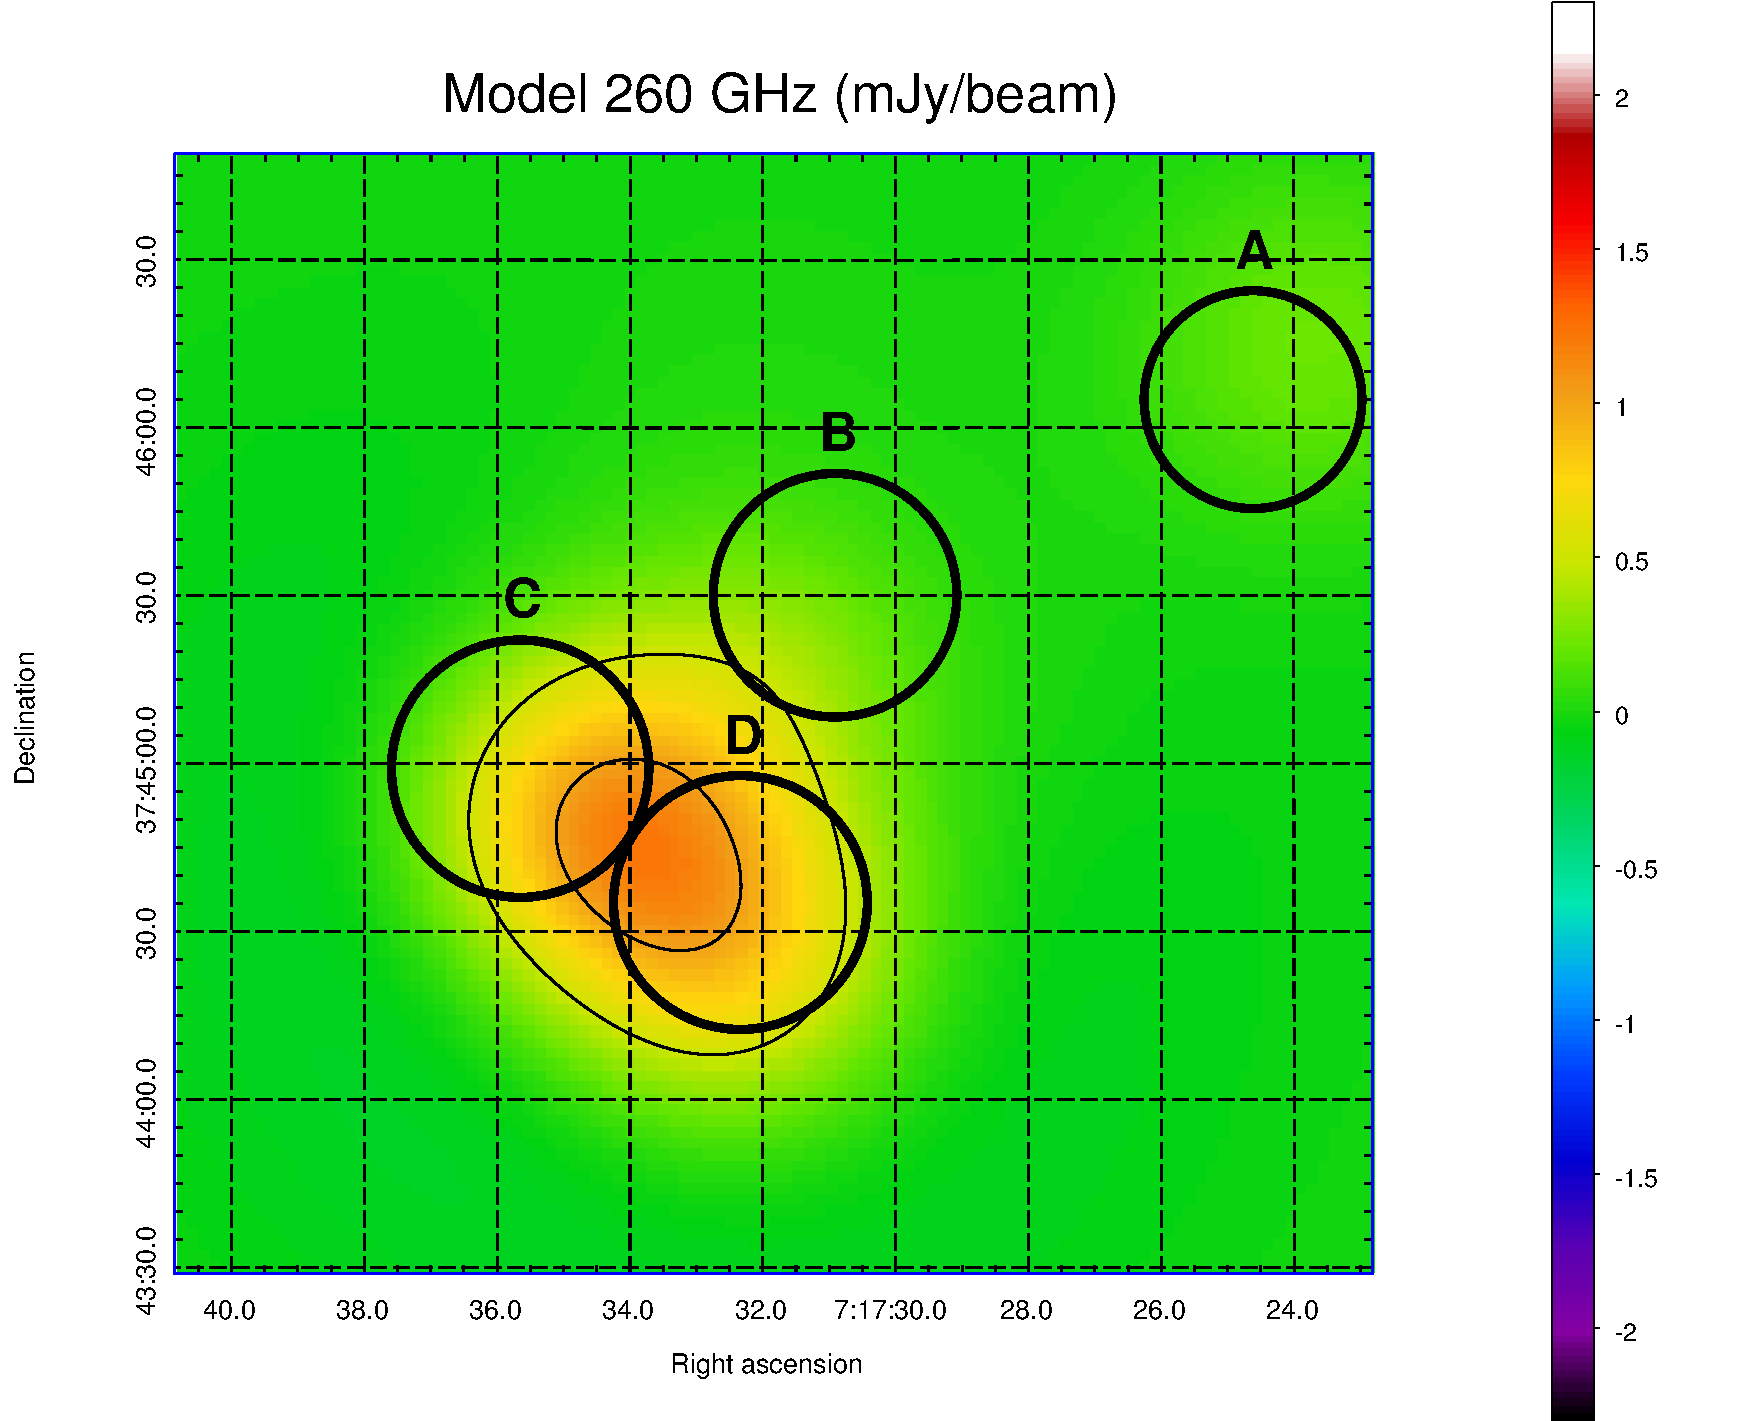
\includegraphics[width=0.42\textwidth]{Model1mm.pdf}
	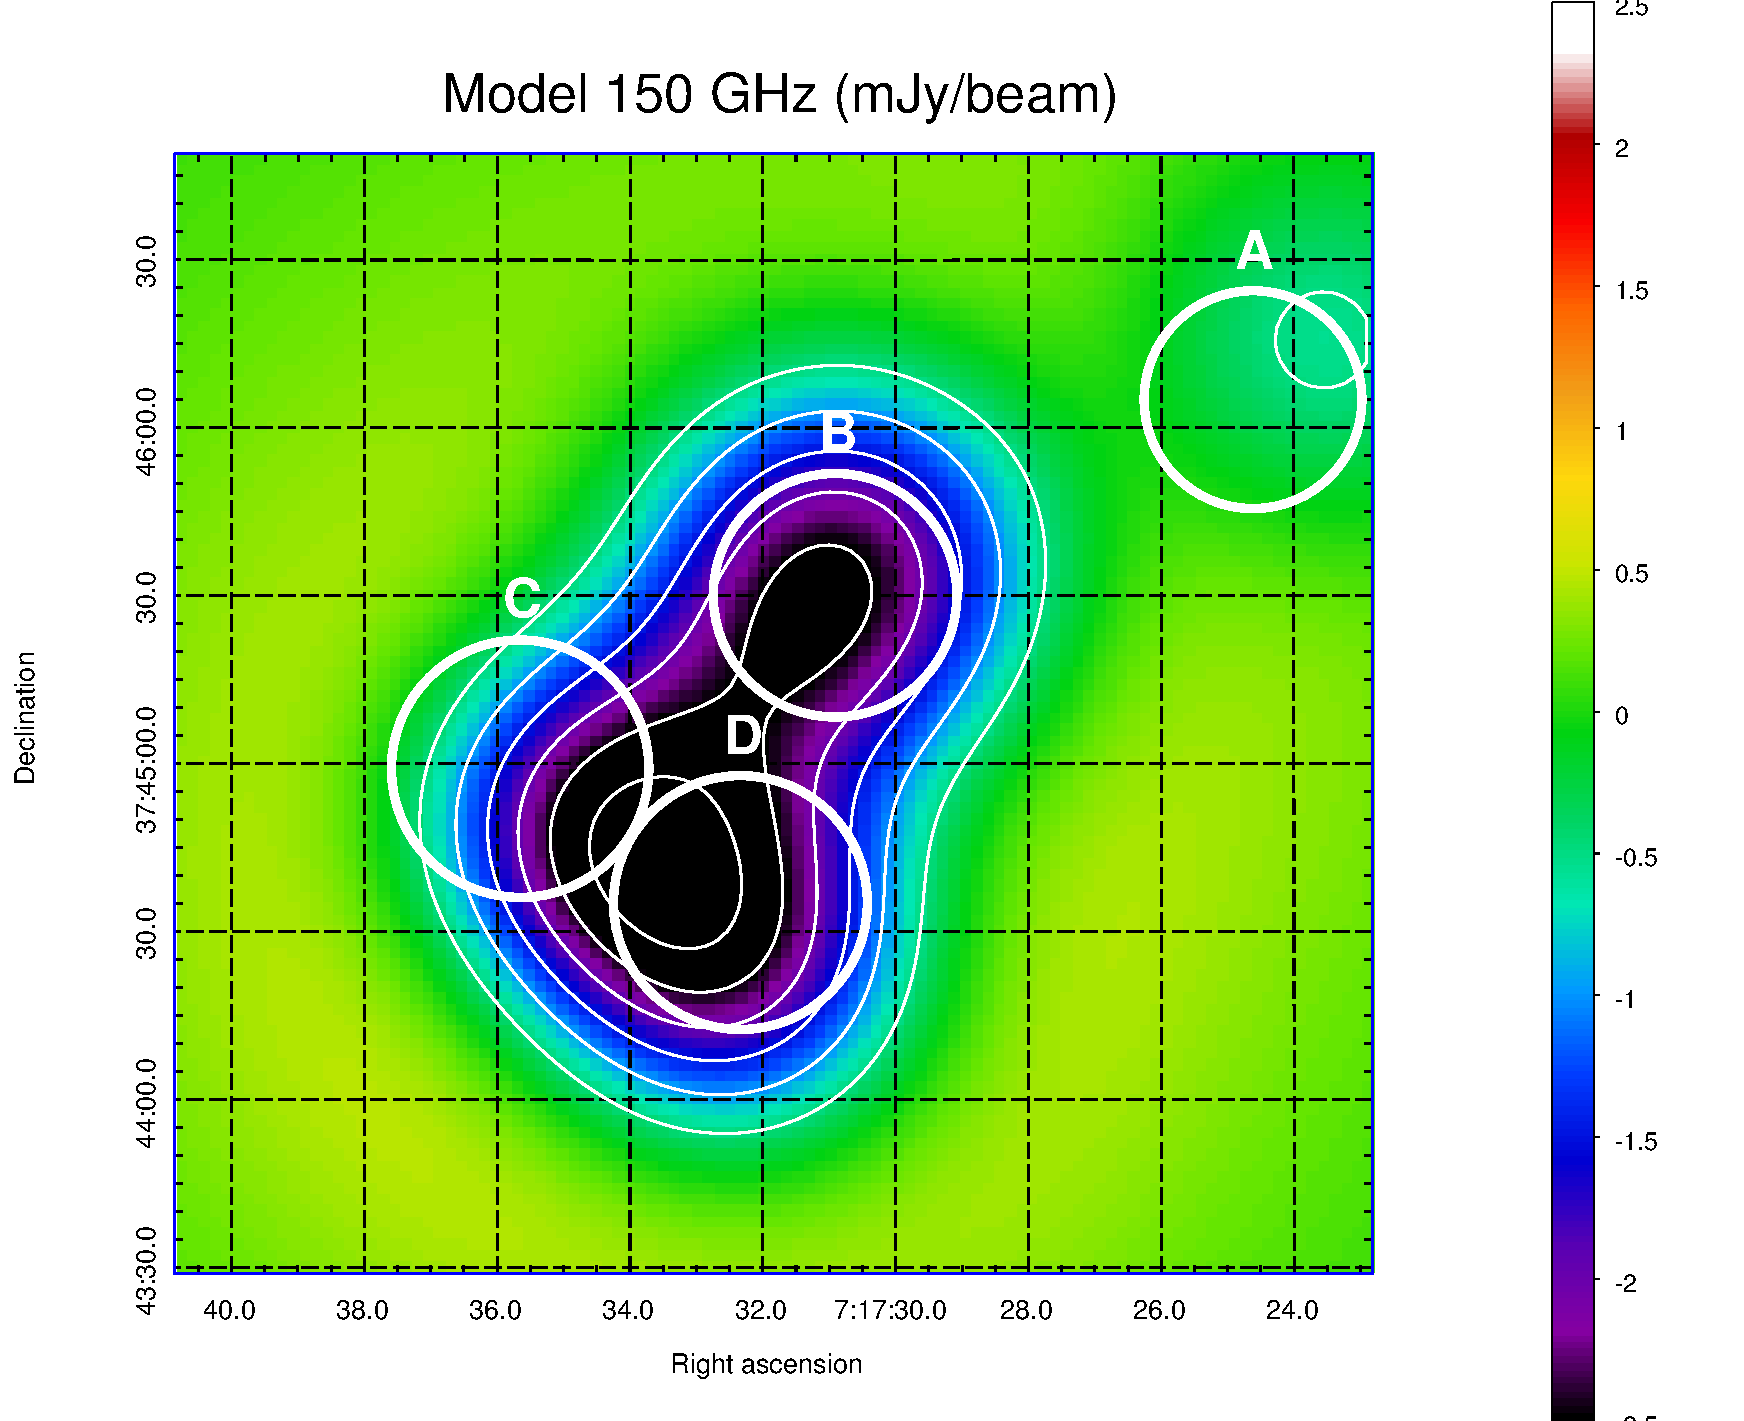
\includegraphics[width=0.42\textwidth]{Model2mm.pdf}
	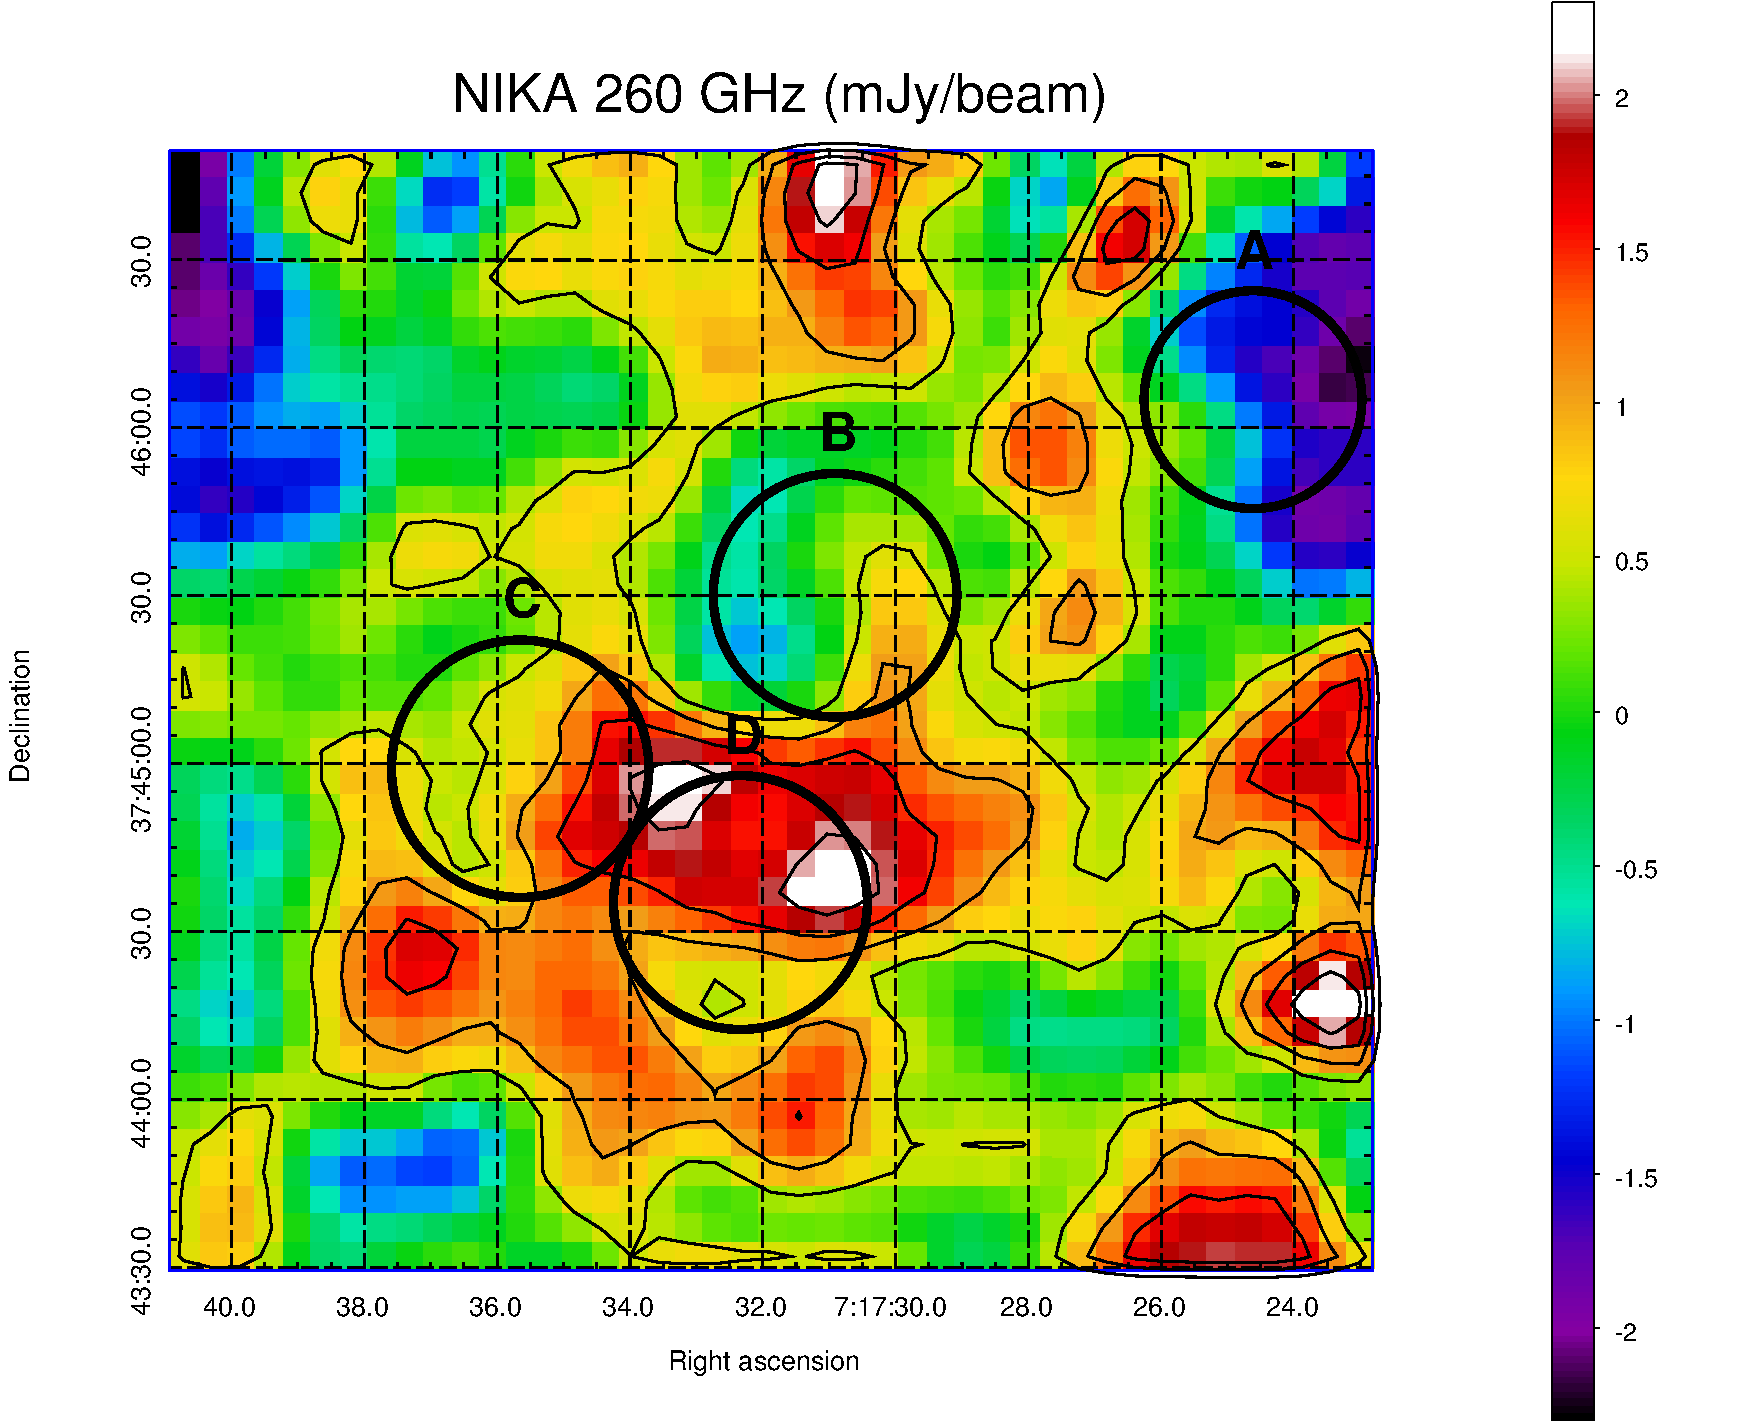
\includegraphics[width=0.42\textwidth]{NIKA1mm.pdf}
	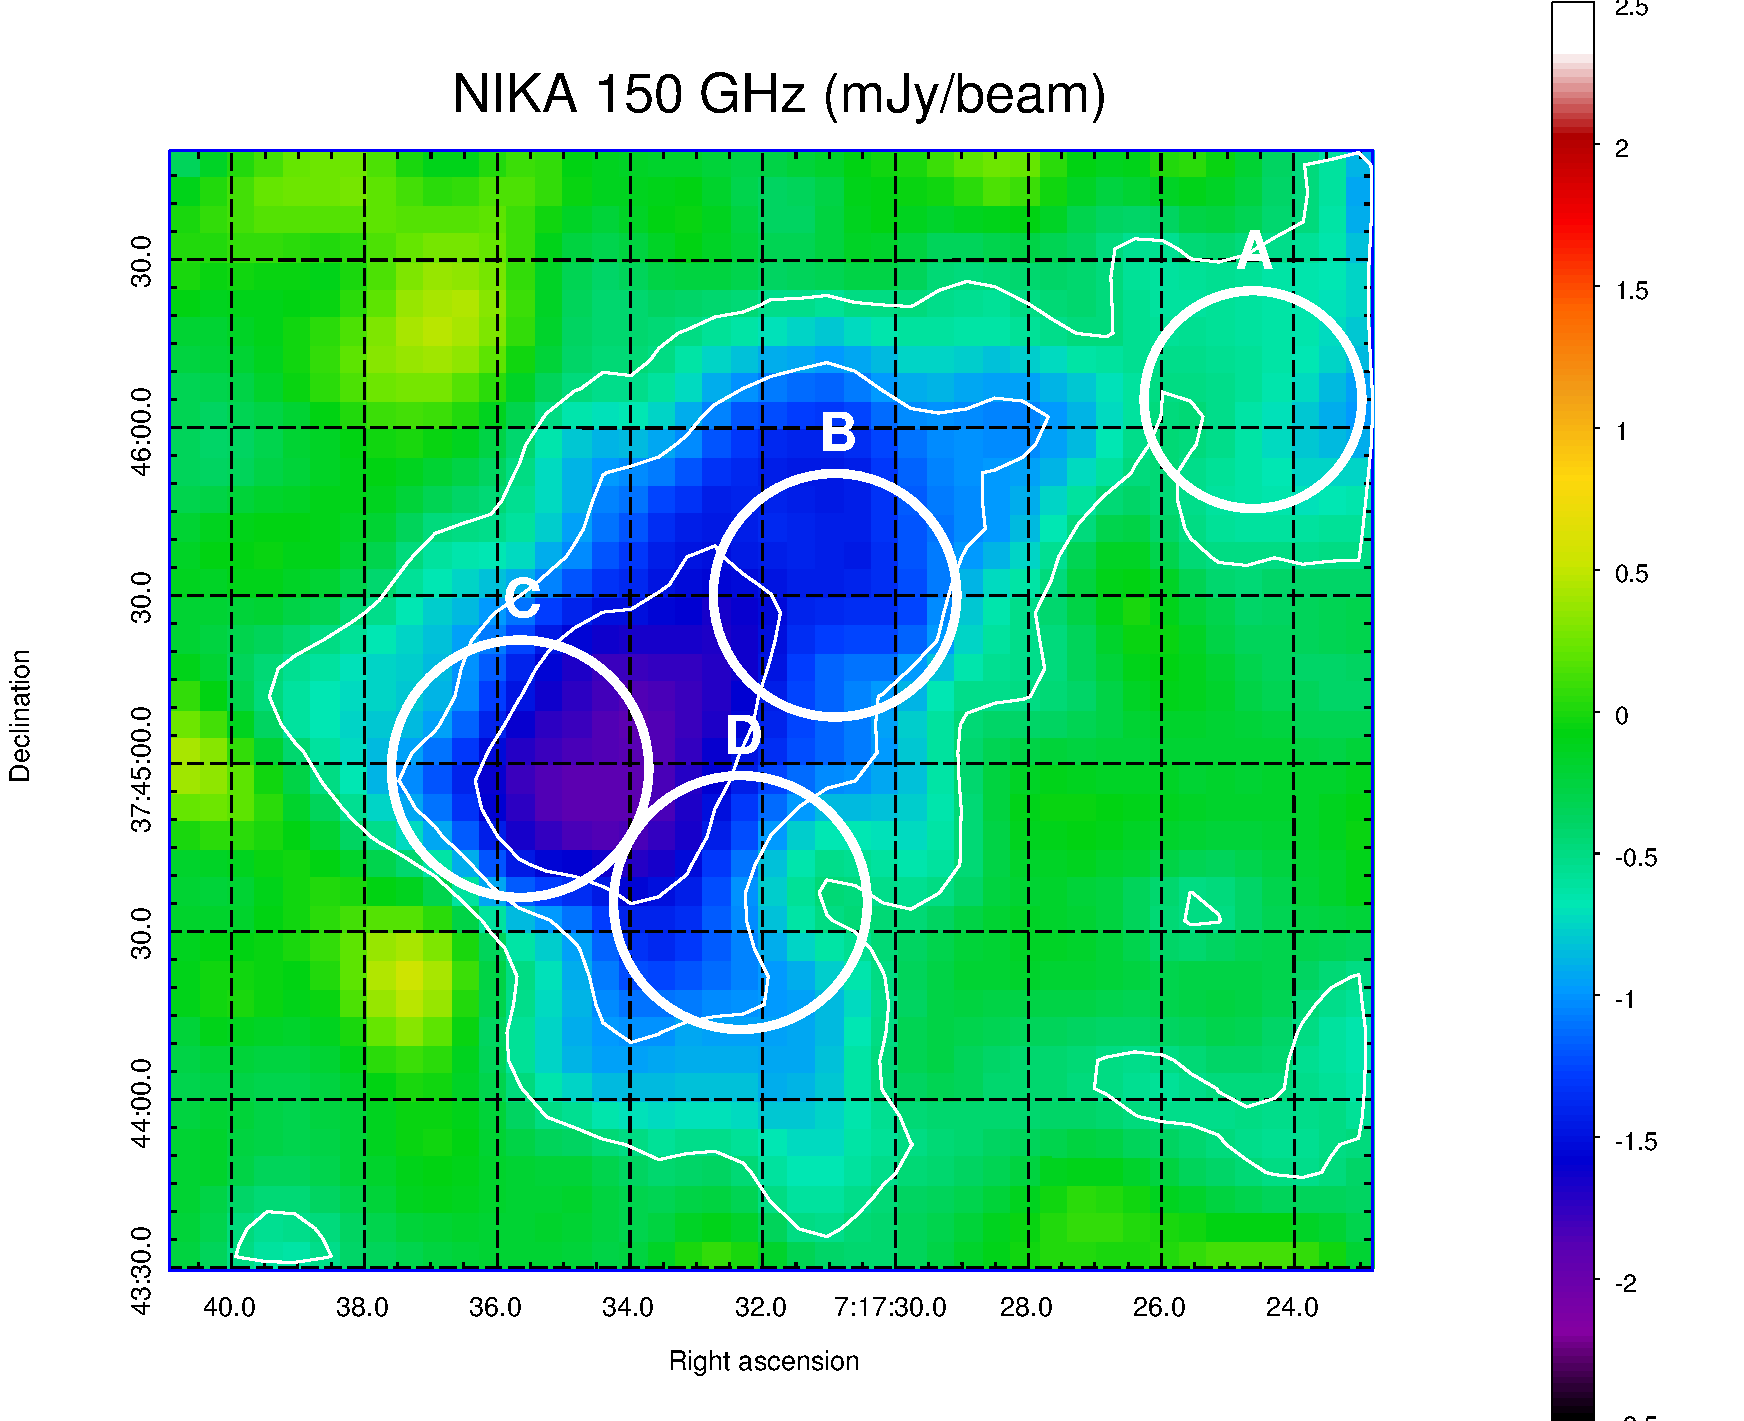
\includegraphics[width=0.42\textwidth]{NIKA2mm.pdf}
	\caption{Multi-wavelength maps of \mbox{MACS~J0717.5+3745} shown on 3.5 arcmin patches. {\bf Top left}: surface mass distribution in units of the critical surface density (convergence, $\kappa$) obtained by \cite{zitrin2009} from Hubble Space Telescope strong lensing observations. Map contours are linearly spaced and highlight the four main optical groups that are also circled by regions from A to D and reproduced on the other panels. {\bf Top right}: \mbox{X-ray} photon counts from Chandra. The image is smoothed to 10~arcsec resolution showing the gas density distribution. Map contours are linearly spaced. While region B is very dense but cold, the temperature in region C and D is extremely high \citep[$\sim$ 30~keV,][]{ma2009}. {\bf Middle row}: simple simulation of the expected tSZ+kSZ signal in the NIKA bands based on optical and \mbox{X-ray} data. Angular scales larger than the NIKA 1.8~arcmin focal plane have been filtered out to account for data processing. The tSZ signal is expected to peak around sub clusters C and D because of the increase in pressure. Concerning the kSZ, it is dominant in region B as it is dense with large line-of-sight velocity (away from the observer). The signal is negative at both frequencies, reinforcing the tSZ signal at 150~GHz and cancelling it out at 260~GHz. \textcolor{gris}{[continuing ...]}}
	\label{fig:maps} 
\end{figure}
\addtocounter{figure}{-1}
\begin{figure} [h!]
  \caption{\textcolor{gris}{[... continuing]} {\bf Bottom}: first NIKA open pool (February 2014) SZ maps at 260~GHZ (left) and 150~GHz (right). The color scales are similar for simulations and data and the SZ contours are spaced by 0.5~mJy/beam steps. The data have been obtained using $\sim$10 hours of observing time, mostly under good atmospheric conditions. Both maps have been smoothed with a 15~arcsec Gaussian filter. At 150~GHz, the SZ signal is extended and appears negative, reaching about 15$\sigma$ at the peak, in region C--D as expected. At 260~GHz, it is positive in region C--D, reaching only 3$\sigma$ as the noise is higher (0.5 mJy/beam $\equiv 1\sigma$ in the central region), but no signal is seen around region B, as expected. More data are necessary to claim a kSZ detection. The general shape of the simulation and the data agree well but the amplitude of the signal seems lower than expected at 150~GHz and higher at 260~GHz.}
\end{figure}
\begin{figure}[h!]
	\centering
	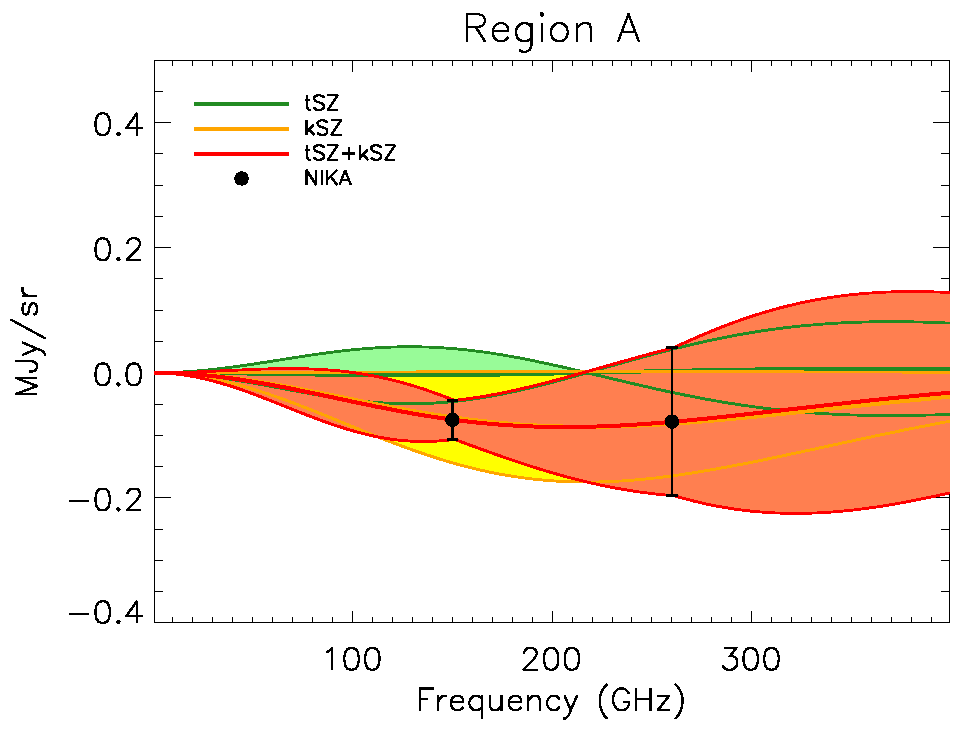
\includegraphics[width=0.39\textwidth]{SZspecA.pdf}
	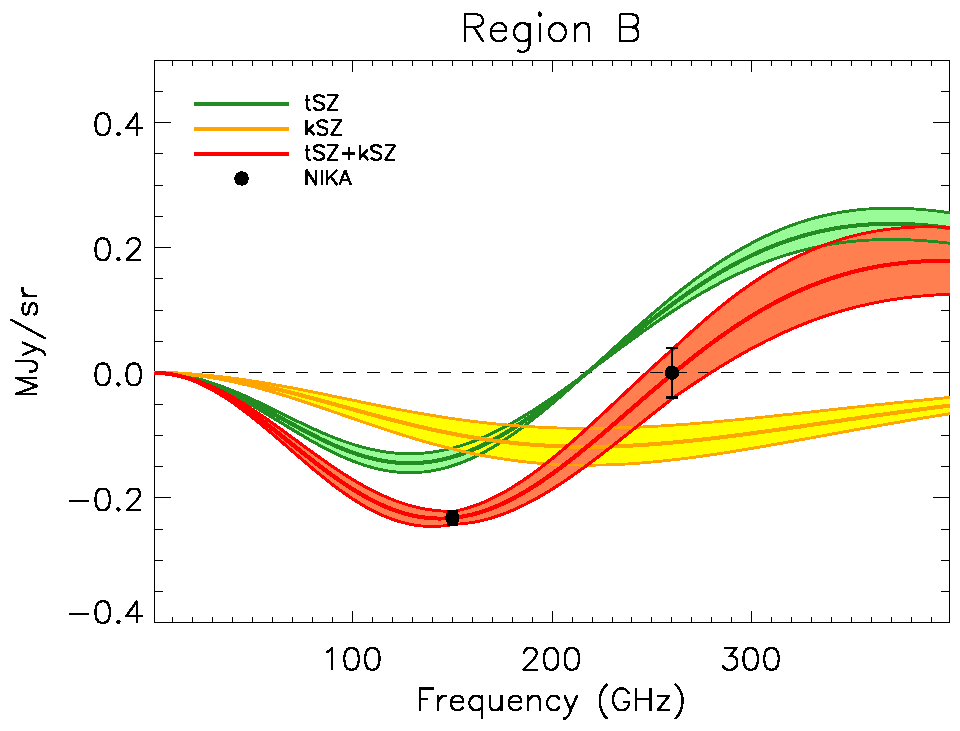
\includegraphics[width=0.39\textwidth]{SZspecB.pdf}
	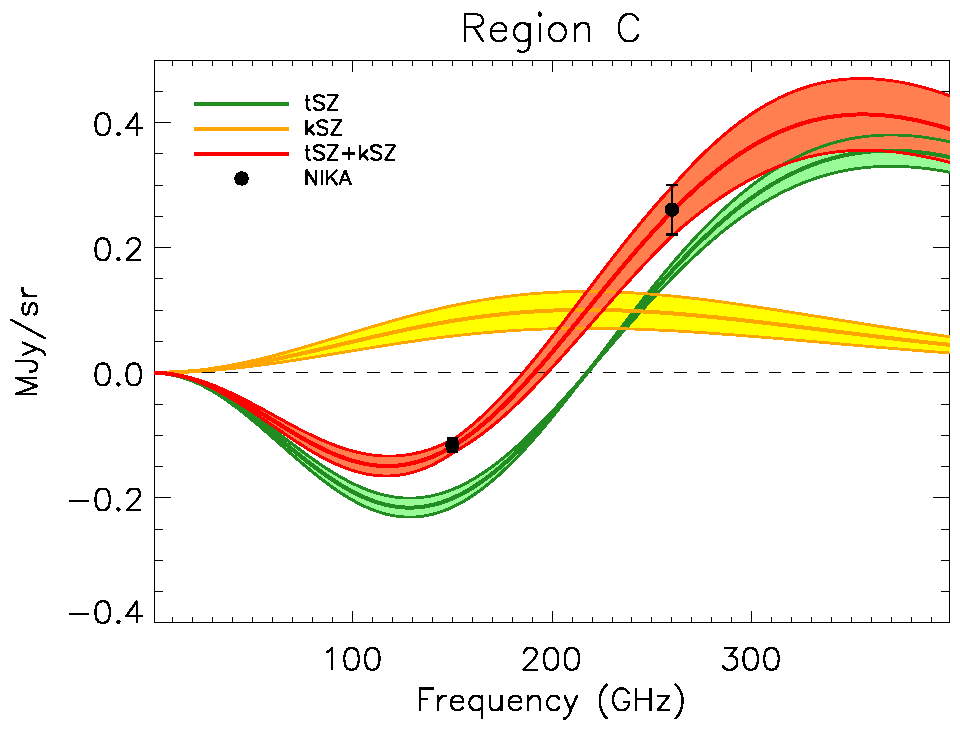
\includegraphics[width=0.39\textwidth]{SZspecC.pdf}
	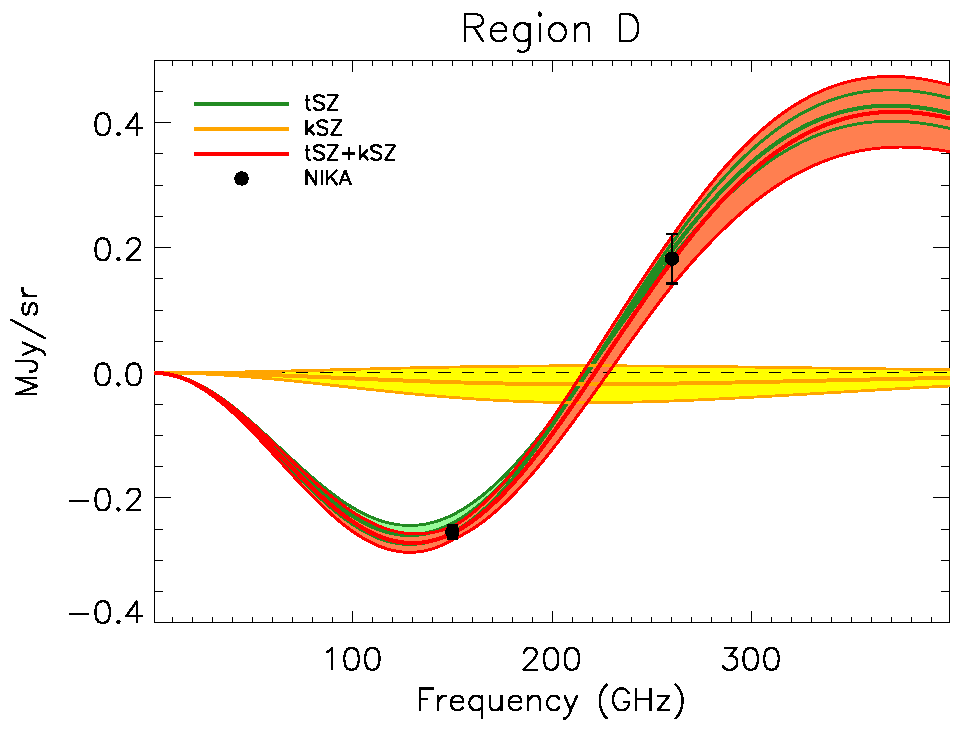
\includegraphics[width=0.39\textwidth]{SZspecD.pdf}
	\caption{Expected constraints on the kSZ+tSZ spectra computed in 22~arcsec pixels towards the four regions shown in Fig.~\ref{fig:maps}, assuming that the NIKA measured flux will remain the same and error bars will reduce according to observing time. The best-fit tSZ+kSZ spectrum is shown in red with 1$\sigma$ error displayed as the red shaded area. Similarly, the individual SZ contributions are given in green (pure thermal) and yellow (pure kinetic). Region A is, and will be, much less constrained as it lies on the edge of the map where the rms of the noise increases by a factor 3. The optical line-of-sight velocities \citep{ma2009} are $278^{+295}_{-339}$ km/s, $3238^{+252}_{-242}$ km/s, $-733^{+486}_{-478}$ km/s, and $831^{+843}_{-800}$ km/s for regions A, B, C and D, respectively.}
	\label{fig:spectra}
\end{figure}

%%%%%%%%%%%%
\begin{thebibliography}{9}

\bibitem[Adam et al.(2013)]{adam2013}
R. Adam, B. Comis, J.-F. Mac\'ias-P\'erez, {\it et al.} (2013), A\&A in press, arXiv:1310.6237
 
\bibitem[Billot et al.(2014)]{billot2014}
N. Billot, \& C. Kramer (2014), http://www.iram.fr/GENERAL/calls/w14/w14.pdf
%http://www.iram.es/IRAMES/mainWiki/Continuum/TimeEstimatorScript

\bibitem[Birkinshaw(1999)]{birkinshaw1999}
M. Birkinshaw (1999), Phys. Rep., 310, 97

\bibitem[Catalano et al.(2014)]{catalano2014}
A. Catalano, M. Calvo, N. Ponthieu, {\it et al.} (2014), A\&A in press, arXiv:1402.0260

\bibitem[Ma et al.(2009)]{ma2009}
C.-J. Ma, H. Ebeling, \& E. Barrett (2009), ApJ, 693, L56

\bibitem[Mroczkowski et al.(2012)]{mroczkowski2012}
T. Mroczkowski, S. Dicker, J. Sayers {\it et al.} (2012), ApJ, 761, 47, arXiv:1205.0052

\bibitem[NIKA col.(2014)]{CL2014}
The NIKA collaboration, {\it et al.} (2014), in prep.
 
\bibitem[Sayers et al.(2013)]{sayers2013}
J. Sayers, T. Mroczkowski, M. Zemcov {\it et al.} (2012), ApJ, 778, 52, arXiv:1312.3680

\bibitem[Ruppin(2013)]{ruppin2013}
F. Ruppin, R. Adam, \& F. Mayet (2013), internal NIKA collaboration note, available upon request
 
\bibitem[Zitrin et al.(2009)]{zitrin2009}
A. Zitrin, T. Broadhurst, Y. Rephaeli, S. Sadeh, {\it et al.} (2009), ApJ, 707, 102

\end{thebibliography}

\end{document}
